%% LaTeX-Beamer template for KIT design
%% by Erik Burger, Christian Hammer
%% title picture by Klaus Krogmann
%%
%% version 2.1
%%
%% mostly compatible to KIT corporate design v2.0
%% http://intranet.kit.edu/gestaltungsrichtlinien.php
%%
%% Problems, bugs and comments to
%% burger@kit.edu

\documentclass[18pt]{beamer}

%% SLIDE FORMAT

% use 'beamerthemekit' for standard 4:3 ratio
% for widescreen slides (16:9), use 'beamerthemekitwide'

\usepackage{templates/beamerthemekit}
\usepackage[utf8]{inputenc}
% \usepackage{templates/beamerthemekitwide}

\usepackage{graphicx}
\usepackage{array}

\setbeamercovered{invisible}

%% TITLE PICTURE

% if a custom picture is to be used on the title page, copy it into the 'logos'
% directory, in the line below, replace 'mypicture' with the
% filename (without extension) and uncomment the following line
% (picture proportions: 63 : 20 for standard, 169 : 40 for wide
% *.eps format if you use latex+dvips+ps2pdf,
% *.jpg/*.png/*.pdf if you use pdflatex)

\titleimage{labor}

%% TITLE LOGO

% for a custom logo on the front page, copy your file into the 'logos'
% directory, insert the filename in the line below and uncomment it

\titlelogo{title}

% (*.eps format if you use latex+dvips+ps2pdf,
% *.jpg/*.png/*.pdf if you use pdflatex)

%% TikZ INTEGRATION

% use these packages for PCM symbols and UML classes
% \usepackage{templates/tikzkit}
% \usepackage{templates/tikzuml}

% the presentation starts here

\title[TruffleHog \& spp\_profinet]{TruffleHog \& spp\_profinet}
%\subtitle{2015}
\author{Maximilian Diez, Mark Giraud, Jan Hermes}

\institute{Fraunhofer IOSB}

% Bibliography

%\usepackage[citestyle=authoryear,bibstyle=numeric,hyperref,backend=biber]{biblatex}
%\addbibresource{templates/example.bib}
%\bibhang1em

\begin{document}

% change the following line to "ngerman" for German style date and logos
\selectlanguage{ngerman}

%title page
\begin{frame}
\titlepage
\end{frame}

%table of contents
\begin{frame}{Gliederung}
\tableofcontents
\end{frame}

\section{Motivation}
    \begin{frame}{Motivation}
    \begin{itemize}[<+->]
      \item Bereich: IT-Sicherheit für Produktionsnetze
      \item Ansatz: Sicherheitssoftware aus Office-Bereich verwenden
      \item Problem: Industrieanlagen verwenden eigene Protokolle
            \newline =$>$ Nicht direkt kompatibel
      \item Erster Schritt: Industrienetzwerk mithören und darstellen
    \end{itemize}
\end{frame} 
\section{Aufgabenstellung}
    \begin{frame}{Aufgabenstellung}
\begin{tabular}{m{8cm}r}
  \textbf{Snort} - Intrusion Detection System
    \begin{itemize}
      \item Paketweise Mitlesen von Netzwerkkommunikation
      \item Suche nach Angriffsmustern
    \end{itemize} & 
\includegraphics[width=0.2\linewidth]{images/max-snort} \\
  \pause
  \textbf{ProfiNet} - Industrielle Ethernet Kommunkation
    \begin{itemize}
      \item Echtzeitfähige Ethernetvariante
    \end{itemize} & 
\includegraphics[width=0.2\linewidth]{images/max-profinet} \\
  \pause
  \textbf{=$>$ Aufgabe:} 
  \begin{itemize} 
    \item Auslesen von ProfiNet-Paketen in Snort und Darstellung des Netzwerks
\end{itemize}
\end{tabular}
\end{frame}

\begin{frame}{Aufgabenstellung}
\begin{figure}
  \centering
  
\includegraphics[width=\textwidth]{./images/aufgabestellung.jpg}
\end{figure}
\end{frame} 
\section{Designentscheidungen}
    \begin{frame}{Einleitung: Anforderungen \& Umsetzung}
    \begin{itemize}
        \item Objektorientierung:
        \begin{itemize}
            \item Snort Plugin: Code in C! Annäherung durch function pointers und structs
            \item Trufflehog: Mit Java 8 kein Problem
        \end{itemize}

        \pause
        \item Modularer Aufbau:
        \begin{itemize}
            \item Baumstruktur für Dissektoren
            \item Trennung von Dissektion und Darstellung
            \pause
            \item Variation des MVC Prinzips
            \item Services
        \end{itemize}
    \end{itemize}
\end{frame} 
\section{Ergebnis}
    \begin{frame}{Ergebnis}
    \begin{center}
    \Huge Programm Demo
    \end{center}
\end{frame} 

\section{Ausblick}
\begin{frame}{Ausblick}
	\begin{tabular}{m{5cm}r}
		Kurzfristig: 5. Phase \vspace{0.5cm} & 
\includegraphics[width=0.3\linewidth]{images/max-junit} \\
		\pause
		Mittelfristig \vspace{0.5cm} & 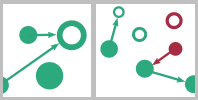
\includegraphics[width=0.2\linewidth]{images/max-tiling} \hspace{0.5cm} 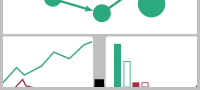
\includegraphics[width=0.2\linewidth]{images/max-stats} \\
		\pause
		Langfristig \vspace{0.5cm} & 
\includegraphics[width=0.2\linewidth]{images/max-snort} \hspace{0.5cm} 
\includegraphics[width=0.2\linewidth]{images/max-profinet} \\
	\end{tabular}
\end{frame}

\begin{frame}
	\centering
	
\includegraphics[width=0.8\linewidth]{images/title}
\end{frame}


\appendix
\beginbackup

%\begin{frame}[allowframebreaks]{References}
%\printbibliography
%\end{frame}

\backupend

\end{document} 